\documentclass[10pt,twocolumn]{article}

\usepackage[margin=0.70in,columnsep=0.24in]{geometry}
\usepackage[T1]{fontenc}
\usepackage{lmodern}
\usepackage{microtype}
\usepackage{amsmath,amssymb}
\usepackage{booktabs}
\usepackage{array}
\usepackage{enumitem}
\usepackage{caption}
\usepackage{tikz}
\usetikzlibrary{positioning,arrows.meta,fit}
\usepackage[hyphens]{xurl}
\usepackage{hyperref}

\hypersetup{
  colorlinks=true,
  linkcolor=black,
  citecolor=black,
  urlcolor=blue,
  pdftitle={A Reproducible Protocol for Evaluating Plastic-Skin Artifacts in Generative Portrait Images},
  pdfauthor={Miles Carter}
}

\setlist[itemize]{leftmargin=1.15em,itemsep=1.5pt,topsep=2pt,parsep=0pt}
\setlist[enumerate]{leftmargin=1.25em,itemsep=1.5pt,topsep=2pt,parsep=0pt}
\captionsetup{font=small,skip=4pt,labelfont=bf}
\emergencystretch=2em
\sloppy
\urlstyle{same}

\newcommand{\prot}{plastic-skin protocol, version~1}

\title{A Reproducible Protocol for Evaluating ``Plastic Skin'' Artifacts in Generative Portrait Images}

\author{%
  Miles Carter\\
  Independent Researcher\\
  \texttt{support@bananaproai.app}%
}

\date{Protocol version 1}

\begin{document}
\maketitle

\begin{abstract}
Generative models produce adult portraits whose global appearance is often convincing while facial skin still reads as wax, airbrushed polymer, or a repeated texture stamp. Distributional image scores, biometric face-image quality, and forensic detector outputs answer different questions, and a smooth cheek can be either a photographic fact or a synthesis failure. This paper specifies the \prot{} for still, photorealistic portraits of adults. The contribution is an operational definition, a seven-family taxonomy grounded in measured skin optics, ordinal severity anchors, a pre-registerable human protocol with sampling strata, negative controls, blinding, and agreement reporting, and a short list of optional instrumental covariates that are explicitly unvalidated. A qualitative walkthrough applies the instrument to three constructed cases. No generator is ranked. The paper reports no new quantitative experiment, no detector accuracy, and no rater-study sample size. A reporting checklist is included so that later studies can be compared without collapsing the phenomenon to a single leaderboard number.
\end{abstract}

\noindent\textbf{Keywords:}
generative portraits;
skin appearance;
evaluation protocol;
human rating;
image forensics;
face-image quality.

\section{Introduction}
\label{sec:intro}

Portrait synthesis has moved from a laboratory demonstration to a routine source of still images. Style-based generative adversarial networks showed that a generator can produce full-frame face photographs with coherent global structure \cite{karras2019stylegan,karras2020stylegan2}. Denoising diffusion and latent diffusion then made text-conditioned and image-conditioned synthesis practical at high resolution \cite{ho2020ddpm,rombach2022ldm,saharia2022imagen,podell2023sdxl}. In that setting, a portrait can be globally plausible and still fail in a narrow, socially salient way: the skin looks like plastic.

``Plastic skin'' is a practitioner name for a family of appearance failures. The cheek is poreless, the highlight is a smooth milky lobe, the ear and the nose lack the local color variation associated with thin tissue and blood, or a pore-like grain repeats as a stamp and then stops at a beard or a hairline. The failure is easy to see in a crop and easy to miss in a score that averages over a whole image or a whole dataset. It is also easy to confuse with phenomena that are photographic. Youth, soft window light, and makeup genuinely reduce visible pores. A protocol that cannot say so will punish real faces, and a protocol that ignores plastic skin will treat a mannequin cheek as a success whenever the eyes, the teeth, and the background geometry look fine.

Existing numbers do not isolate the failure. The Fr\'echet Inception Distance and the Inception Score summarize a set of images in a classifier feature space \cite{heusel2017fid,salimans2016is}. Precision and recall variants ask whether samples fall on the data manifold and whether they cover it \cite{sajjadi2018pr,kynkaanniemi2019pr}. Those quantities can move because of background clutter, cropping, or an aliased resize \cite{parmar2022alias,borji2019}. Likelihood and visual fidelity can come apart in high dimension \cite{theis2016note}. Biometric face-image quality asks whether a sample is useful for recognition \cite{schlett2022,iso29794}. Forensic classifiers ask whether a generator left a detectable trace \cite{wang2020cnn,verdoliva2020}. A face can score well on all three tests and still look waxen, or it can look like skin and remain forensically detectable. Perceptual studies have already shown that observers sometimes judge synthetic faces to be human, and even judge them as more trustworthy than photographs \cite{nightingale2022,miller2023}. Those studies answer a detection question. They do not hand a laboratory a scoring procedure for skin.

This paper specifies a procedure that a laboratory can run later. It does not run that procedure. The specification has five parts.
\begin{enumerate}
  \item An operational definition of plastic skin and a seven-family taxonomy tied to interface reflection, mesostructure, and subsurface transport, together with the confounds that must be flagged rather than scored as failures.
  \item Ordinal severity anchors and a scoring rule that keeps the overall grade equal to the maximum family grade, so that laboratories do not invent private averages.
  \item A human protocol: who may be depicted, how stimuli are stratified and blinded, how raters are trained, how two viewing passes work, which agreement statistics are reported, and which claims are out of bounds.
  \item Optional instrumental covariates, written as hypotheses with definitions and with an explicit statement that no threshold in this paper is a validated detector.
  \item A reporting checklist, a metadata dictionary, and a rater card.
\end{enumerate}
A qualitative walkthrough in Section~\ref{sec:walk} shows how the rater card is filled for three constructed cases. Those marks are teaching annotations. They are not measurements.

The protocol is deliberately narrower than ``does this portrait look real.'' Extra fingers, malformed jewelry, broken background perspective, and illegible text are recorded in a side channel so that they do not inflate a skin grade. Video, non-human characters, stylized illustration, and any image that appears to depict a minor are out of scope. Absence of plastic skin is not evidence that a person in the image exists, and presence of plastic skin is not evidence of deceptive intent.

\section{Related work}
\label{sec:related}

\subsection{Portrait generators and the factors a protocol must record}

Generative adversarial networks learn a sampler by a game between a generator and a discriminator \cite{goodfellow2014gan}. Progressive and style-based architectures made high-resolution face synthesis stable enough that the residual errors shifted from global incoherence toward texture, aliasing, and dataset bias \cite{karras2019stylegan,karras2020stylegan2,karras2021stylegan3}. The alias-free redesign in particular treats texture sticking and upsampling artifacts as first-class signal-processing faults \cite{karras2021stylegan3}. Diffusion models define synthesis as the reversal of a noise process \cite{ho2020ddpm}. Latent diffusion and later text-to-image systems run that reversal in a learned latent space under language conditioning \cite{rombach2022ldm,saharia2022imagen,podell2023sdxl}.

Classifier-free guidance mixes a conditional score estimate with an unconditional one and thereby exposes a fidelity--diversity tradeoff that the sampler, not only the training set, controls \cite{ho2022cfg}. Guidance scale, step count, sampler, resolution, seed, prompt text, and negative prompt are therefore metadata of the stimulus, on the same footing as lens and lighting metadata for a photograph. Version~1 of the protocol records them and does not assume that any particular setting produces plastic skin. Establishing that link would be a separate, pre-registered experiment.

Neural function classes are biased toward lower spatial frequencies \cite{rahaman2019spectral}. Upsampling stacks in convolutional generators have been shown to distort spectra relative to natural images \cite{durall2020upconv,frank2020freq,chandrasegaran2021}. Those results motivate a suspicion that mesostructure will be the first thing a generator gets wrong. They do not define the perceptual failure, and they do not justify a universal frequency threshold. Section~\ref{sec:instrument} explains what a laboratory may compute, and what it may not claim.

\subsection{Why dataset-level scores do not answer the question}

Borji's survey of evaluation measures makes the practical point that no single scalar captures the ways a generator can fail \cite{borji2019}. Theis, van den Oord, and Bethge showed that log-likelihood, a Parzen-window estimate, and the visual quality of samples can be largely independent in high dimension, so success on one criterion does not transfer to another \cite{theis2016note}. FID depends on the feature extractor and on seemingly minor preprocessing; aliased resizing alone can reorder model comparisons \cite{heusel2017fid,parmar2022alias}. Precision and recall assess manifold membership and coverage \cite{sajjadi2018pr,kynkaanniemi2019pr}. LPIPS and SSIM compare images that are already aligned \cite{zhang2018lpips,wang2004ssim}. BRISQUE and NIQE predict generic naturalness deviations from statistical regularities of photographs \cite{mittal2012brisque,mittal2013niqe}. A CLIP embedding can score text--image agreement because the embedding was trained to pair images with captions \cite{radford2021clip}. None of these instruments isolates facial skin, and a gain on any of them is compatible with a worse cheek.

Otani and colleagues surveyed human evaluations of text-to-image models and found that many papers either skipped human rating or described it too loosely to repeat, and that automatic measures in their pilot collection did not stand in for human judgments \cite{otani2023}. Version~1 follows that methodological moral for a narrower target. The primary record is a blinded human grade under a frozen rubric. Automatic features, when used, are covariates.

\subsection{Perception of synthetic faces}

Mori's uncanny-valley essay, in the widely used English translation, describes affinity falling as an artificial figure approaches a human appearance and then recovering when the figure becomes fully convincing \cite{mori2012}. Nightingale and Farid reported that StyleGAN2 faces had, in their experiments, reached a regime in which observers did not reliably separate them from photographs, and in which the synthetic faces were rated slightly more trustworthy \cite{nightingale2022}. Miller and colleagues replicated a stronger pattern for White faces, which they call AI hyperrealism: White StyleGAN2 faces were classified as human more often than the matched photographs, observers who were most often wrong were not correspondingly uncertain, and lay reports plus a face-space analysis identified attributes that people misuse \cite{miller2023,valentine1991}. In their regression, faces rated as more smooth-skinned were judged human less often. Smoothness is already a folk cue.

That finding is a reason to write a skin protocol with care, rather than a reason to equate smoothness with synthesis. Miller and colleagues measured perceived smoothness as one attribute among others. They did not separate makeup, age, illumination, and generator oversmoothing, and they did not propose a physical cutoff. Version~1 treats that separation as the measurement problem. It also treats hyperrealism as a warning about validity: if raters are told that an image is synthetic before they score the skin, the folk cue will leak into the grade. Blinding is part of the measurement, not a courtesy.

Face-space theory supplies a second warning. Generators trained to reproduce the densest part of a training distribution tend to produce faces that are unusually average \cite{valentine1991,karras2020stylegan2,miller2023}. Averageness can look like cleanliness of skin. A protocol that scores only global ``realness'' will mix that demographic and statistical central tendency with the local optical failure. The families in Section~\ref{sec:taxonomy} are local on purpose.

\subsection{Skin as a measured material}

Human skin is not a painted Lambertian surface. Interface reflection at the oily surface and body reflection from the translucent tissue have different spectra and different geometry; Shafer's dichromatic model is the classical statement of that split for dielectric surfaces \cite{shafer1985}. A practical subsurface-transport model made translucent materials, including skin, renderable from first principles \cite{jensen2001}. Later measurement work fitted spatially varying reflectance and scattering on real faces and showed that the parameters change across the face and with age, sex, skin type, makeup, and transient factors such as sweat and cold \cite{weyrich2006,donner2008}. Igarashi, Nishino, and Nayar survey the optical and anatomical structure that those models approximate: a thin, rough, partially oily surface over a layered tissue in which melanin and hemoglobin dominate absorption \cite{igarashi2007}.

Three consequences follow for evaluation. First, pores, fine lines, and vellus hair are mesostructure. They modulate both the specular field and the apparent color. Erasing them is a specific edit, not a generic loss of sharpness. Second, chromophore concentration is spatially organized. The ear, the ala of the nose, and the transition toward the lip carry color variation that a single albedo coat does not. Third, specular energy on a face is uneven. A large, smooth highlight on a cheek, disconnected from microgeometry, is optically unlike the small, broken specularities of oily skin. Version~1 names the corresponding failure families F1--F3 and F2 in particular. It does not claim that a rater mentally inverts a bidirectional reflectance distribution. It claims that the families are specific enough to be pointed at.

Fitzpatrick phototypes were designed for sun reactivity in dermatology \cite{fitzpatrick1988}. They are a weak coordinate system for the appearance of skin in a photograph. The Monk Skin Tone scale is a ten-point appearance scale intended for that different job \cite{monk2019}. Version~1 uses Monk bands as a sampling stratum. The stratum is an appearance label under the study display, not a race label and not a clinical measurement. Intersectional error in face analysis is already documented when appearance is collapsed carelessly \cite{buolamwini2018}. FairFace is relevant here as a reminder that face datasets need an explicit demographic design \cite{karkkainen2021fairface}. Version~1 requires skin-tone balance and records any additional demographic scheme as optional and ethics-approved, rather than requiring raters to assign race.

\subsection{Forensics and biometric quality}

A separate literature asks whether a synthetic image can be detected. Early work exploited blinking, head-pose inconsistency, and visual glitches around eyes, teeth, and facial boundaries \cite{matern2019}. Large manipulated-face datasets made supervised detection a benchmark problem \cite{rossler2019}. Generator-specific fingerprints, spectral irregularities, and autocorrelation patterns distinguish many CNN samples from photographs, and similar regularities have been reported for diffusion samples, including differences in mid- and high-frequency energy \cite{yu2019fingerprint,durall2020upconv,frank2020freq,wang2020cnn,corvi2023icassp,corvi2023cvprw}. Verdoliva's survey places these tests in the broader forensic setting \cite{verdoliva2020}. Wang and colleagues emphasized the fragility of a detector trained on one generator family with the phrase ``for now'' \cite{wang2020cnn}. Compression, resizing, and a new sampler move the forensic feature. A perceptual rubber cheek can also be produced by a generative edit of a real photograph, in which case the global fingerprint story is the wrong story.

Biometric sample quality, including the face-image standard ISO/IEC~29794-5:2025 and the research surveyed by Schlett and colleagues, estimates utility for comparison and enrollment \cite{iso29794,schlett2022,terhorst2020serfiq}. A sharp, frontal, evenly lit mannequin can be a high-utility biometric sample. Version~1 is not a quality algorithm in that sense and should not be reported as one.

\subsection{Reporting precedents}

Datasheets and model cards argue that datasets and models need a structured account of provenance, intended use, and limitations \cite{gebru2021,mitchell2019}. Preregistration separates the analysis that was planned from the analysis that was suggested by the outcomes \cite{nosek2018}. Subjective image quality already has a mature discipline of viewing conditions, rating scales, and observer screening in ITU-R~BT.500-15 \cite{itu500}. Inter-rater statistics have their own failure modes: an unspecified intraclass correlation is not interpretable, and reliability limits the power of any later test that averages raters \cite{shrout1979,koo2016,hallgren2012,hayes2007}. Version~1 borrows the habits of those literatures: freeze the rubric, record the viewing conditions, name the agreement coefficient, and publish deviations. It does not borrow a television-impairment scale as if skin plasticity were a coding artifact.

\section{Failure taxonomy}
\label{sec:taxonomy}

\subsection{Operational definition}

In this protocol, plastic skin is an appearance property of visible facial skin and of neck skin in the same frame. It is present when the skin reads as a molded polymer, a wax surface, or an airbrushed layer whose spatial structure is inconsistent with the lighting, the visible age cues outside the skin, and the anatomy of the region being inspected. The property is graded by family. It is not a binary certificate that an image is synthetic, and it is not a judgment of attractiveness.

The definition is intentionally photographic. A physically based renderer can aim at the same surface and can be scored with the same card. A painterly or anime portrait is out of scope because the intended material is not a photograph of skin. If a study wishes to score stylization leakage inside an otherwise photorealistic portrait, it pre-registers that extension as a separate family and does not silently fold it into F1.

\subsection{Seven families}

Families may co-occur. Raters assign each family its own grade. They do not pick a single ``main'' artifact and ignore the others.

\begin{description}[style=nextline,leftmargin=1.4em,itemsep=2pt,topsep=2pt]
  \item[F1. Mesostructure erasure.]
  Pores, fine lines, and vellus hair are missing on a region where the resolution and the light would show them in a photograph of comparable framing. The surface looks sanded. Sharp hair edges elsewhere in the frame are evidence against explaining the whole image as defocus.
  \item[F2. Plastic specular lobe.]
  The highlight is a large, smooth, low-detail lobe, often milky, and it is not broken by microgeometry. A shiny nose with a quieter cheek is ordinary oiliness \cite{weyrich2006}. The failure pattern is spatial smoothness of the specular field, especially when the cheek is shinier and smoother than the nose.
  \item[F3. Subsurface and chromophore flattening.]
  Color looks like a single coat. Local redness at the ear or the nasal ala, and the gradual transition of color at the lip margin, are missing, in tension with layered skin models \cite{donner2008,igarashi2007}. A uniform pale, orange, or gray cast belongs here when it replaces spatial pigment variation rather than when the entire photograph has a white-balance shift. A global cast is noted as a capture confound.
  \item[F4. Boundary discontinuity.]
  Texture, sharpness, or color changes abruptly at the hairline, beard, glasses, nostril rim, jaw, or the boundary between face and neck, as if two materials had been composited. Ordinary occlusion contours are not discontinuities.
  \item[F5. Stamped or replicated texture.]
  High-frequency grain is present, so the region would not be described as blurry, but the grain repeats, ignores curvature and pore flow, or tiles across the cheek. This family exists so that a residual-energy statistic cannot be mistaken for a pass.
  \item[F6. Geometry-insensitive illumination.]
  Skin shading disagrees with the geometry of the face: concavities lack self-shadowing while the hair obeys another light, or the cheek highlight and the nasal shadow imply different sources. The rater scores skin shading only. Broken background perspective is a side-channel note.
  \item[F7. Age or expression incoherence of skin markings.]
  Non-skin cues indicate an age or an expression that the skin markings contradict. A broad smile with no change whatever in the cheek fold or the periocular skin can qualify. Hair color, a caption, or a rater's guess about a person's age does not qualify. When non-skin cues are absent, F7 is left at zero. Inferring age from the smoothness of the skin and then penalizing that smoothness is circular, and version~1 forbids it.
\end{description}

Figure~\ref{fig:optics} maps the optical groups to the families that most directly violate them. F4, F5, and F7 are structural and semantic rather than single-layer optical faults, which is why a purely spectral detector is the wrong primary instrument.

\begin{figure}[t]
\centering
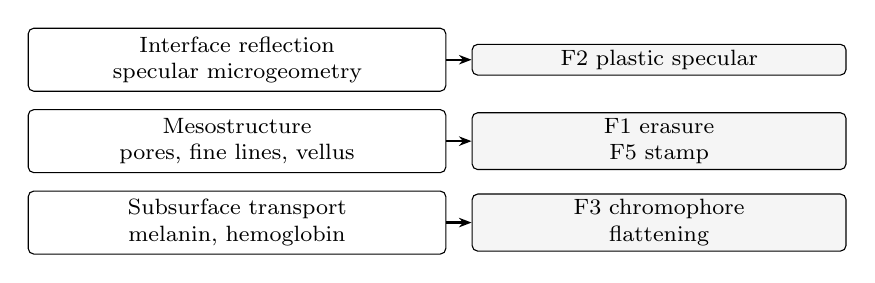
\begin{tikzpicture}[
  font=\footnotesize,
  layer/.style={draw, rounded corners=2pt, align=center, inner sep=3pt, text width=0.42\linewidth, minimum height=8mm},
  fam/.style={draw, rounded corners=2pt, align=center, inner sep=2pt, text width=0.38\linewidth, fill=gray!8}
]
  \node[layer] (a) {Interface reflection\\specular microgeometry};
  \node[layer, below=2.2mm of a] (b) {Mesostructure\\pores, fine lines, vellus};
  \node[layer, below=2.2mm of b] (c) {Subsurface transport\\melanin, hemoglobin};
  \node[fam, right=3.2mm of a] (fa) {F2 plastic specular};
  \node[fam, right=3.2mm of b] (fb) {F1 erasure\\F5 stamp};
  \node[fam, right=3.2mm of c] (fc) {F3 chromophore\\flattening};
  \draw[-{Stealth[length=1.6mm]}, thick] (a.east) -- (fa.west);
  \draw[-{Stealth[length=1.6mm]}, thick] (b.east) -- (fb.west);
  \draw[-{Stealth[length=1.6mm]}, thick] (c.east) -- (fc.west);
\end{tikzpicture}
\caption{Schematic correspondence between skin-optics layers and the families that violate them. F4, F6, and F7 are not drawn: they are boundary, illumination, and semantic inconsistencies across regions. The drawing is not a rendering and not a stimulus.}
\label{fig:optics}
\end{figure}

\subsection{What the rater does not call plastic skin}

The following are confound flags, not families. A flag can accompany a grade. It does not automatically zero the grade, and it does not automatically raise it.
\begin{itemize}
  \item Makeup, including matte foundation, when pores remain at sites where makeup is usually thinner, such as the nasal ala, the ear, or the hairline.
  \item Soft focus or shallow depth of field, when edges that should be in the focal plane are soft together with the skin.
  \item Resolution below the pre-registered floor (Section~\ref{sec:protocol}).
  \item Compression blocking, banding, or oversharpening halos.
  \item Dermatological appearance, including burns, occlusive dressings, and conditions that legitimately alter texture. Raters are not asked to diagnose. They flag ``dermatological uncertainty'' and avoid a high grade unless the plastic pattern is independent of the uncertain region.
  \item A global color grade or film emulation applied to the whole frame.
\end{itemize}
Anatomical faults outside skin, including teeth, eyes as organs, jewelry, hands, and background geometry, go to the side channel. An extra finger does not raise F1.

\subsection{Severity anchors and the overall grade}

Each family is graded on a five-point ordinal scale. The anchors are verbal so that a laboratory can translate them only by issuing a named new version.
\begin{itemize}
  \item \textbf{0, absent.} The family is not visible at the inspection resolution.
  \item \textbf{1, trace.} Visible only during the close inspection pass, and only in a small part of a region.
  \item \textbf{2, localized.} Visible at the intended display size in one facial zone, while other zones still show photographic skin structure.
  \item \textbf{3, extensive.} The family dominates most of the visible facial skin, or, for F4 and F5, the defect is obvious at display size and extends across a region boundary.
  \item \textbf{4, mannequin.} For F1--F3 and F5, facial skin reads as plastic, wax, doll, or an obvious tile across essentially all visible zones. For F4, F6, and F7, the inconsistency makes the skin as a material impossible to reconcile with the rest of the head.
\end{itemize}
When a rater hesitates between two adjacent grades, the lower grade is assigned and confidence is marked low. This bias is conservative and is part of the instrument. It will under-call borderline cases. Studies that want a symmetric rule may pre-register one; the default of version~1 is the lower grade.

The overall grade is the maximum of the seven family grades. It is a reporting convenience. Means of ordinal grades may be published only as descriptive statistics beside the full distribution. A confirmatory endpoint that dichotomizes the scale uses the anchor boundary ``extensive or mannequin,'' that is, overall grade at least~3, unless another cut is pre-registered with a justification. The paper does not estimate how often any generator exceeds that cut.

Figure~\ref{fig:rois} names the inspection regions. The order is fixed so that raters do not skip ears and necks, which are disproportionately informative for F3 and F4.

\begin{figure}[t]
\centering
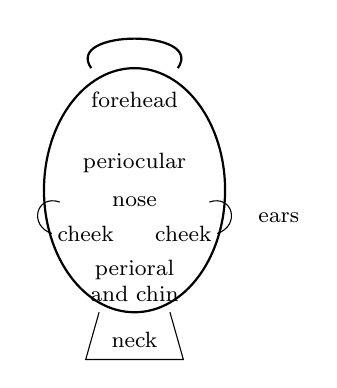
\begin{tikzpicture}[font=\footnotesize, every node/.style={align=center}]
  \draw[thick] (0,0) ellipse (1.15 and 1.55);
  \draw[thick] (-0.55,1.55) .. controls (-0.9,2.05) and (0.9,2.05) .. (0.55,1.55);
  \draw (-0.95,-0.15) .. controls (-1.25,-0.05) and (-1.35,-0.45) .. (-1.05,-0.55);
  \draw (0.95,-0.15) .. controls (1.25,-0.05) and (1.35,-0.45) .. (1.05,-0.55);
  \draw (-0.45,-1.55) -- (-0.62,-2.15) -- (0.62,-2.15) -- (0.45,-1.55);
  \node at (0,1.15) {forehead};
  \node at (0,0.35) {periocular};
  \node at (0,-0.15) {nose};
  \node at (-0.62,-0.55) {cheek};
  \node at (0.62,-0.55) {cheek};
  \node at (0,-1.15) {perioral\\and chin};
  \node at (0,-1.9) {neck};
  \node[anchor=west] at (1.45,-0.35) {ears};
\end{tikzpicture}
\caption{Inspection order for the close pass: forehead and hairline, both cheeks, nose including the alae, perioral skin and chin, visible ears, jawline and neck, then periocular skin. The eye itself is not scored as skin. Schematic only.}
\label{fig:rois}
\end{figure}

\section{Evaluation protocol}
\label{sec:protocol}

\subsection{Status of the defaults}

Every numeric default in this section is an administrative choice that makes two laboratories comparable if they both adopt version~1 unchanged. None of the defaults is a fitted optimum. A laboratory may pre-register a deviation before any outcome is examined. A deviation chosen after the grades are known is reported as such and is not described as confirmatory \cite{nosek2018}.

\subsection{Who and what may be included}

The protocol scores still images with a photorealistic intent that depict adults. Images that appear to depict minors are excluded before rating, whether or not the image is sexual, and they are not placed in the calibration pack. If age is ambiguous, the image is excluded. Non-consensual intimate imagery is out of scope. The protocol is an evaluation instrument for appearance, not a production aid.

A face enters the rated set only if facial skin is visible and the interocular distance in the rated file is at least 64 pixels. Below that administrative floor, pore-scale structure is not available to the rater and a plastic-skin grade becomes a resolution grade. Laboratories that need a stricter floor, for example a minimum cheek-crop size, pre-register it. Images rejected by the screen are counted in the checklist, not dropped silently.

Source types are \emph{real}, \emph{generated}, and \emph{edited}. Edited means a real photograph passed through a generative or parametric retouch, restoration, or relighting operation. The visual rubric does not depend on source type. The analysis may stratify on it after unblinding.

\subsection{Sampling frame}

Stimuli are stratified so that a single easy cell cannot dominate the distribution. The required factors are:
\begin{itemize}
  \item Monk Skin Tone appearance band, estimated visually on facial skin under the study display. A study pre-registers how the ten points collapse into bands. A recommended collapse for balance targets, not a biological claim, is light (1--3), medium (4--6), and dark (7--10).
  \item Adult age-appearance band, using cues other than skin smoothness: for example 18--30, 31--50, 51--70, and over~70. The bands label appearance for sampling. They are not identity attributes.
  \item Lighting: diffuse window, hard sun, studio, low light, colored practical light.
  \item Pose: frontal, three-quarter, profile.
  \item Expression: neutral, smile, other.
  \item Occlusion: none, facial hair, eyeglasses, hair over the forehead.
  \item Source type, and, for generated and edited images, model family.
\end{itemize}
Empty cells are reported empty. Sex presentation may be balanced as an appearance factor. It is not inferred as a biological attribute, and a study that adds a gender or race label says whose label it is and under what instruction \cite{buolamwini2018}. Version~1 does not require race labels.

Generators and prompts are frozen before rating. The prompt list is hashed, and the hash is part of the preregistration. Seeds, exact model versions, guidance scales, samplers, step counts, resolutions, and edit operations are metadata (Appendix~\ref{app:meta}). A public prompt collection may be archived as that list. Archiving a list is not a claim about the list.

\subsection{Reference photographs and controls}

Real references are photographs that the laboratory has the right to use for the study. Acceptable sources include newly captured images with documented consent and existing collections whose license and consent status have been reviewed in writing. Scraping private social-media accounts is not a source this protocol endorses. Widely used research face sets, including sets built from celebrity photographs and from Flickr, raise consent and redistribution issues that the laboratory's ethics review has to confront explicitly \cite{karras2019stylegan,lee2020celebamask}. A face parser, if used later for a covariate, may be trained on region labels of the kind released with CelebAMask-HQ \cite{lee2020celebamask}. Parser errors are an exclusion reason for the covariate, not for the human grade. The human grade does not require a parser.

Three kinds of controls are required.
\begin{enumerate}
  \item \textbf{Ordinary photographs,} including unretouched faces with visible pores, across the skin-tone bands.
  \item \textbf{Legitimately smooth photographs,} including makeup and soft light, so that smoothness alone is not diagnostic. These are negative controls for the plastic-skin label.
  \item \textbf{Attention constructions,} made from licensed photographs by a documented transformation. The two constructions specified by version~1 are a Gaussian smooth applied only inside a skin mask, and a clone of a small skin patch laid in a grid on the cheek. The first should attract a non-zero F1 grade. The second should attract a non-zero F5 grade. They are process checks. They are not portraits from any named generator, and they are not an endpoint.
\end{enumerate}
If attention items can cause a rater to be excluded, the exclusion rule is pre-registered. A rule consistent with the instrument is to flag for review any rater who assigns F1\,=\,0 to a masked-smooth attention item. Version~1 does not convert that flag into an automatic rejection quota.

\subsection{Blinding, order, and display}

Filenames are hashed. Model names are removed from the rating interface. Real, generated, edited, and attention items are interleaved. Raters are not told the base rate. Each rater receives a distinct order. The person who holds the blinding key does not rate.

Display conditions are reported in the spirit of a subjective-quality experiment \cite{itu500}: monitor model and diagonal size, viewing distance, room light, sRGB or another named profile, and whether a colorimeter was used. Version~1 does not require a colorimeter. A study without one says so. The rated pixels are the file that was hashed. An extra beauty pass, an extra sharpen, or a recompression that is not in the metadata invalidates the grade.

Viewing has two passes. In the global pass, the image is shown at the intended size for 6 seconds with zoom disabled. The rater does not grade during the 6 seconds. In the inspection pass, zoom and panning are allowed, regions are visited in the order of Figure~\ref{fig:rois}, and only then is the card filled. The 6-second value is a default so that the global impression is sampled before pixel hunting. It is not a claim about reaction time.

\subsection{Raters and calibration}

Raters are adults. Two pools are defined, and they are not mixed in one reliability coefficient unless the analysis of pool is pre-registered: naive observers, and practitioners who retouch or generate portraits as part of their work. Expertise is a factor. It is not treated as ground truth. A dermatologist panel is welcome and is not required by version~1.

Each image is graded independently by at least three raters, so that disagreement is observable. That minimum makes disagreement visible. It does not by itself yield a precise reliability estimate \cite{hallgren2012}. Studies that need a tight confidence interval on agreement use more raters and say why.

The calibration pack is frozen, disjoint from the study set, and contains at least one intended positive example and one confound counterexample for each family. The laboratory may build positives from the attention constructions and from images it has the right to alter. Raters discuss disagreements on the calibration pack before any study image is graded. The discussion is minuted. Version~1 does not set a numeric cutoff for dismissing a rater. A laboratory that wants one pre-registers it.

\subsection{The rating tasks}

The primary task is the family card: seven ordinal grades, seven opportunities to set a confound flag, a three-level confidence mark (low, medium, high) for the image as a whole, and a short free-text note. Confidence is stored and is not multiplied into the grade. The dissociation between confidence and accuracy reported for synthetic-face detection is exactly why confidence stays a separate column \cite{miller2023}.

The free-text note catches failures outside the taxonomy. Notes are coded in a later pass. A note does not change a grade unless it names a missed skin family, in which case the image is re-rated under a documented adjudication rule and both the original and the revised grades are retained.

An optional paired task applies when the scientific question is an edit. The before image and the after image are graded independently under blinding. Pairing is revealed at analysis. The primary within-pair summary, if pre-registered, is the distribution of the difference in overall grade, with the reliability of each side.

Figure~\ref{fig:flow} is the order of operations. Analysis that starts before the rubric, the prompt hash, and the exclusion rules are frozen is exploratory even if the arithmetic is correct.

\begin{figure}[t]
\centering
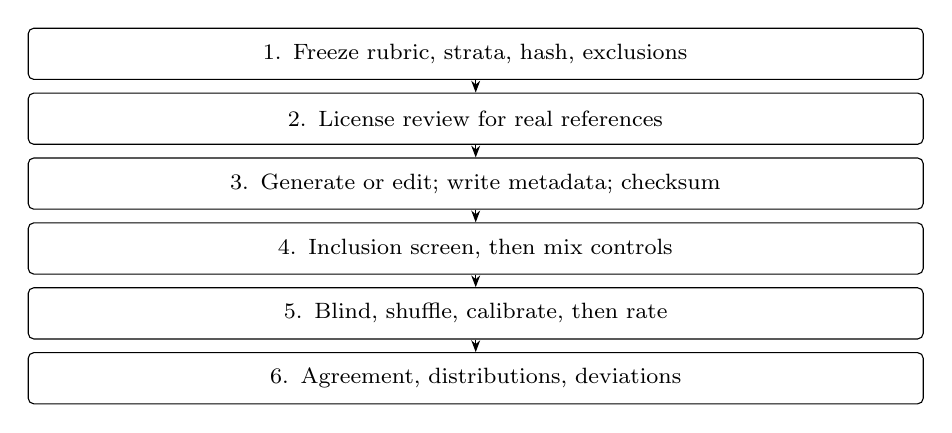
\begin{tikzpicture}[
  font=\footnotesize,
  box/.style={draw, rounded corners=2pt, align=center, inner sep=3pt, text width=0.92\linewidth, minimum height=6.5mm}
]
  \node[box] (a) {1. Freeze rubric, strata, hash, exclusions};
  \node[box, below=1.6mm of a] (b) {2. License review for real references};
  \node[box, below=1.6mm of b] (c) {3. Generate or edit; write metadata; checksum};
  \node[box, below=1.6mm of c] (d) {4. Inclusion screen, then mix controls};
  \node[box, below=1.6mm of d] (e) {5. Blind, shuffle, calibrate, then rate};
  \node[box, below=1.6mm of e] (f) {6. Agreement, distributions, deviations};
  \draw[-{Stealth[length=1.5mm]}] (a) -- (b);
  \draw[-{Stealth[length=1.5mm]}] (b) -- (c);
  \draw[-{Stealth[length=1.5mm]}] (c) -- (d);
  \draw[-{Stealth[length=1.5mm]}] (d) -- (e);
  \draw[-{Stealth[length=1.5mm]}] (e) -- (f);
\end{tikzpicture}
\caption{Order of operations for a study that claims conformance with version~1. The diagram is a checklist in graphical form, not a system architecture.}
\label{fig:flow}
\end{figure}

\subsection{Agreement, endpoints, and claims that are out of bounds}

The primary descriptive product is the distribution of overall grades and of each family grade, stratified at least by skin-tone band and by source type. Cell counts accompany every stratum. Reliability is a co-primary report. For ordinal family grades the default coefficient is Krippendorff's alpha with an ordinal difference function \cite{hayes2007}. If a laboratory reports an intraclass correlation instead, it names the form, the software, and whether the coefficient is for a single rater or for the average, as required for the number to be interpretable \cite{shrout1979,koo2016}. Landis and Koch's bands for kappa are conventions only; version~1 does not treat them as pass--fail lines for publication \cite{landis1977,cohen1960}.

If the range of overall grades on one image is at least~3 points, the image is flagged. A consensus discussion may be held and must be stored separately from the independent grades. The independent grades remain the primary record. The flag threshold is an administrative rule.

A confirmatory comparison of named systems is allowed only as a pre-registered secondary analysis. It reports full distributions, strata, reliability, and the metadata of Appendix~\ref{app:meta}. It uses a pre-registered error-rate control if more than one contrast is tested. Version~1 does not include a sample-size formula. A confirmatory study powers its own endpoint, states the smallest effect that would matter, and treats rater variance as part of the design \cite{hallgren2012}. Planned sample size is fixed before rating.

The following sentences are not licensed by conformance to the protocol, and this paper does not assert them: that a named model is the best portrait system; that a lower FID implies cleaner skin; that a forensic detector's accuracy equals a plastic-skin rate; that a high biometric-quality score implies photographic skin; that absence of plastic skin shows the person exists; that presence of plastic skin shows fraud.

\subsection{Optional instrumental covariates}
\label{sec:instrument}

A laboratory may attach covariates computed on a skin mask. They are hypotheses. They do not override the human grade, and version~1 publishes no operating threshold.

Let \(Y\) be relative luminance after the file's transfer function is inverted to linear light, using the standard sRGB coefficients \(Y = 0.2126\,R + 0.7152\,G + 0.0722\,B\) when the working space is sRGB. Let \(R\) be the set of mask pixels in one facial region, and let \(G_{\sigma}\) be a Gaussian low-pass whose scale \(\sigma\) is frozen in the preregistration. The residual energy
\begin{equation}
  e(R) = \frac{1}{|R|}\sum_{p \in R}\bigl(Y(p) - (G_{\sigma} * Y)(p)\bigr)^{2}
  \label{eq:energy}
\end{equation}
measures whether mid-frequency variation is present. It does not measure whether that variation is anatomical. Case~B in Section~\ref{sec:walk} is the counterexample: a stamp can raise \(e(R)\) while failing F5. Darker skin under the same exposure often yields lower high-frequency contrast for optical reasons already modeled by melanin absorption \cite{igarashi2007,donner2008}. A single global cutoff on \(e(R)\) would therefore confuse tone with texture. Version~1 forbids that cutoff. If \(e(R)\) is reported, it is reported as a distribution within skin-tone band, or as a paired difference against a licensed photograph of similar framing, and the mask failure rate is reported beside it.

A second hypothesis, motivated by the dichromatic split \cite{shafer1985}, concerns the specular field. Candidate highlight pixels are those that are bright and whose chromaticity has moved toward the estimated illuminant. The covariate is the size distribution of connected components of that set inside \(R\). The hypothesis is that a plastic lobe tends to form one large component, whereas oily skin tends to form many small ones. No component-size cutoff is given.

A third hypothesis concerns replication. For a cheek patch \(P\) and a shift \(\delta\), the normalized cross-correlation \(c(\delta)\) between \(P\) and its shift has a peak at the origin by construction. A secondary peak at a small nonzero shift is a reason for a human to look again for F5. It is not itself a grade.

A fourth hypothesis compares \(e\) on the cheek with \(e\) on the ear. Measured faces are not uniformly textured \cite{weyrich2006}. A global smoothness prior can make those regions too similar. The pair is descriptive.

These four quantities may be useful in a later measurement study. Publishing them without the human distribution, the strata, and the mask failure rate is not conformance.

\subsection{Ethics of use}

Grades describe images under a rubric. They are not findings about a real person's character, health, or truthfulness. Publishing a grade beside an identifiable individual's photograph requires a basis that the appearance protocol itself does not supply. Raters are told that synthetic faces can look ordinary and still be misused, so a low plastic-skin grade is not a verification of identity \cite{nightingale2022}. Compensation, consent, and review by the relevant ethics body are the laboratory's obligations. Version~1 is not an ethics determination.

Rater pools have their own biases. Studies report voluntary aggregate information about the pool and do not treat a single demographic of raters as a universal observer. Makeup norms differ by place and period. The calibration pack for a deployment context should include local examples of ordinary cosmetic practice so that F1 is not a penalty for foundation. That adaptation is a documented variant, not a silent change.

\section{Worked qualitative walkthrough}
\label{sec:walk}

This section applies the card to three constructed cases. The cases are verbal stimuli, written so that a reader can see which family moves and which stays still. They are not outputs of a named system, they were not shown to a rater panel, and the marks in Table~\ref{tab:teach} are one author's teaching annotations. A citation that treats the table as a result is a misuse of the paper.

\begin{table*}[t]
\centering
\caption{Teaching annotation of three constructed cases. Entries are ordinal labels under Section~\ref{sec:taxonomy}, assigned by the author to the verbal stimuli in Section~\ref{sec:walk}. They are not measurements, inter-rater statistics, or model scores.}
\label{tab:teach}
\footnotesize
\begin{tabular}{@{}lccc@{}}
\toprule
Family & Case A, wax cheek & Case B, stamp & Case C, makeup \\
\midrule
F1 mesostructure erasure & extensive & absent & trace \\
F2 plastic specular & extensive & absent & absent \\
F3 chromophore flattening & localized & absent & absent \\
F4 boundary discontinuity & absent & localized & absent \\
F5 stamped texture & absent & extensive & absent \\
F6 illumination & trace & absent & absent \\
F7 age or expression & absent & absent & absent \\
Makeup confound & no & no & yes \\
Overall grade (maximum) & extensive & extensive & trace \\
\bottomrule
\end{tabular}
\end{table*}

\textbf{Case A, wax cheek.}
The global pass shows a symmetrical adult headshot under soft studio light. Hair edges are sharp, the two eyes point consistently, and the background is a plain sweep. Nothing in the six-second impression forces a skin grade, which is why the global pass is not the rating. On the inspection pass the cheek highlight is a single soft ellipse of constant hue, unbroken by pores. The nasal ala and the visible ear are the same flat color as the cheek, without the local blood variation those regions usually carry. The nose is less shiny than the cheek. Hair at the temple does not smear into the forehead, so F4 stays absent. A slight mismatch between the cheek highlight and the shadow under the chin is enough for F6 at trace, not more, because the geometry is otherwise coherent. Non-skin age cues are not in conflict with the skin, so F7 stays absent. The maximum is extensive, driven by F1 and F2. A FID computed on a mixed dataset could still be small if the global face distribution were close to the reference set. That possibility is a reason the protocol exists. It is not a FID, and none is reported.

The negative control for Case A is a photograph of makeup under similar light in which the cheek is smooth, the nose still carries broken specularities, and the ear still shows local redness. That control is how a rater learns not to copy the Case A grades onto every matte cheek. The protocol's instruction is to grade the control on what remains inexplicable after the makeup flag, not to grade the genre ``portrait of a made-up person.''

\textbf{Case B, stamp.}
The cheek is full of fine grain, so an honest computation of Equation~\eqref{eq:energy} would not describe the region as empty. The grain repeats at a nearly constant offset, does not follow the crease beside the nose, and ends in a hard line where the beard begins. F1 is therefore absent: the failure is not erasure. F5 is extensive because the replication is obvious at display size across the cheek. F4 is localized to the beard boundary and does not by itself dominate the head. F2 and F3 stay absent because the highlight is broken and the ear still differs in color from the cheek. The overall grade is extensive because the maximum rule follows F5. The case is in the protocol so that a laboratory tempted to replace the rater card with residual energy has a qualitative counterexample on the page. No energy value is computed here, because no image is filed with the paper.

\textbf{Case C, legitimate makeup.}
The global pass shows a young adult by a window, with visible cosmetics. On inspection, cheek pores are reduced and the forehead is matte, but pores remain beside the nasal ala, the ear is redder than the cheek, the neck matches the jaw, and the specular field is stronger on the nose than on the cheek. F1 is trace rather than absent, because a small sanded patch is visible on the cheekbone during the close pass, and the makeup flag is set. Every other family is absent. The lower-grade rule matters: a rater who hesitates between absent and trace on F1 chooses trace only if the sanded patch is actually seen, and otherwise chooses absent. The teaching mark uses trace in order to show the flag and the grade coexisting. A later consensus discussion might move that single family to absent. Under version~1 the independent mark would still be kept. The scientific point is the decision, not the trace label. Case C is a success of the protocol when the rater refuses to treat cosmetics as a mannequin.

Across the three cases the same overall word, ``extensive,'' arises for different families. A leaderboard that stored only the overall grade would identify Case A with Case B. The family vector is the result a study keeps. The overall grade is the maximum, reported beside the vector, and it is never the only column in the archive.

\section{Limitations}
\label{sec:limits}

Version~1 is unvalidated. No rater panel has used the card, no agreement coefficient has been computed, and no generator has been scored. The anchors may be too coarse, or too fine, once real raters apply them. Families may need to be split or merged. That work is a measurement study, and this paper is the instrument that such a study can freeze.

The taxonomy is conservative about scope. It does not score hands, teeth, or hair except where hair forms a boundary with skin. It does not score video. Temporal failures, including texture that sticks under motion or swims across frames, are related to aliasing concerns already studied for generators \cite{karras2021stylegan3} and need a separate protocol with a defined clip length and a playback size. Applying still-image grades to isolated frames of a video will miss those failures and can also double-count a single bad shot.

Several judgments remain soft. F7 depends on non-skin cues that can themselves be synthetic. The instruction to leave F7 at zero when those cues are missing will cause misses. The makeup flag depends on the rater's familiarity with cosmetic practice. A calibration pack built in one country will under-prepare raters in another. English anchors will not survive an undocumented translation. A translated card is a new version string.

Instrumental covariates inherit the biases of the mask and of exposure. Equation~\eqref{eq:energy} is not comparable across skin tones without stratification. Connected-component summaries of highlights depend on the illuminant estimate, which a colored practical light can defeat. Version~1 therefore keeps the human grade primary.

The protocol can be gamed if a training loss is written to minimize predicted grades. Publishing the rubric makes that easier. The appropriate response is to treat the rubric as an evaluation instrument that is re-validated when generators change, not as a permanent feature extractor. Forensic experience already shows that detector features move when generators move \cite{wang2020cnn,corvi2023icassp}. Plastic-skin grades will move as well.

Finally, the author is an independent practitioner. No dermatologist co-author, no multi-site rater study, and no funded data collection stand behind the defaults. Readers should adopt the 64-pixel floor, the 6-second global pass, the three-rater minimum, and the range-of-three flag as conventions of this version, and they should replace them openly if evidence warrants a version~2.

\section{Conclusion}
Plastic skin is a local failure of portrait synthesis and of generative retouching. It is visible, it is socially legible, and it is poorly matched to the scalars that currently dominate generator papers. The \prot{} makes the failure specific: seven families, verbal anchors, a maximum rule for the overall grade, a sampling frame that treats skin tone and lighting as design factors, blinded two-pass rating, negative controls for ordinary smoothness, attention constructions for erasure and stamping, and a checklist that forbids substituting FID, biometric quality, or a forensic score for the grade.

The paper stops where a specification should stop. It does not estimate how common the failure is, which system produces it, or how often raters agree. Those are properties of future studies that freeze this version, or that publish a later version with deviations marked. Until such studies exist, the honest summary of the evidence in this document is qualitative. The taxonomy is grounded in skin optics and in prior perceptual and forensic work, and the procedure is concrete enough to run, criticize, and replace.

\section*{Acknowledgments}
The author is responsible for the taxonomy, the protocol, the citations, and the decision to report no empirical performance numbers. A text-to-text generative AI system assisted with outlining, drafting, and language editing. No text-to-image model was used to create figures; the diagrams are TikZ drawings specified for this manuscript. Generative AI is not an author.

The correspondence address uses the same domain as the implementation named in Appendix~\ref{app:resources}. That appendix is a resource pointer. This paper does not evaluate the implementation and states no performance claim about it.

\begin{thebibliography}{99}
\scriptsize

\bibitem{goodfellow2014gan}
I.~Goodfellow, J.~Pouget-Abadie, M.~Mirza, B.~Xu, D.~Warde-Farley, S.~Ozair, A.~Courville, and Y.~Bengio.
Generative adversarial nets.
In \emph{Advances in Neural Information Processing Systems (NIPS)}, 2014.

\bibitem{karras2019stylegan}
T.~Karras, S.~Laine, and T.~Aila.
A style-based generator architecture for generative adversarial networks.
In \emph{Proc.\ IEEE/CVF Conf.\ Computer Vision and Pattern Recognition (CVPR)}, 2019.

\bibitem{karras2020stylegan2}
T.~Karras, S.~Laine, M.~Aittala, J.~Hellsten, J.~Lehtinen, and T.~Aila.
Analyzing and improving the image quality of {StyleGAN}.
In \emph{Proc.\ IEEE/CVF Conf.\ Computer Vision and Pattern Recognition (CVPR)}, 2020.

\bibitem{karras2021stylegan3}
T.~Karras, M.~Aittala, S.~Laine, E.~H{\"a}rk{\"o}nen, J.~Hellsten, J.~Lehtinen, and T.~Aila.
Alias-free generative adversarial networks.
In \emph{Advances in Neural Information Processing Systems}, 2021.

\bibitem{ho2020ddpm}
J.~Ho, A.~Jain, and P.~Abbeel.
Denoising diffusion probabilistic models.
In \emph{Advances in Neural Information Processing Systems}, 2020.

\bibitem{rombach2022ldm}
R.~Rombach, A.~Blattmann, D.~Lorenz, P.~Esser, and B.~Ommer.
High-resolution image synthesis with latent diffusion models.
In \emph{Proc.\ IEEE/CVF Conf.\ Computer Vision and Pattern Recognition (CVPR)}, 2022.

\bibitem{saharia2022imagen}
C.~Saharia, W.~Chan, S.~Saxena, L.~Li, J.~Whang, E.~Denton, S.~K.~S.~Ghasemipour, B.~K.~Ayan, S.~S.~Mahdavi, R.~G.~Lopes, T.~Salimans, J.~Ho, D.~J.~Fleet, and M.~Norouzi.
Photorealistic text-to-image diffusion models with deep language understanding.
In \emph{Advances in Neural Information Processing Systems}, 2022.

\bibitem{podell2023sdxl}
D.~Podell, Z.~English, K.~Lacey, A.~Blattmann, T.~Dockhorn, J.~M{\"u}ller, J.~Penna, and R.~Rombach.
{SDXL}: Improving latent diffusion models for high-resolution image synthesis.
arXiv:2307.01952, 2023.

\bibitem{ho2022cfg}
J.~Ho and T.~Salimans.
Classifier-free diffusion guidance.
arXiv:2207.12598, 2022.
A short version appeared at the NeurIPS 2021 Workshop on Deep Generative Models and Downstream Applications.

\bibitem{rahaman2019spectral}
N.~Rahaman, A.~Baratin, D.~Arpit, F.~Draxler, M.~Lin, F.~Hamprecht, Y.~Bengio, and A.~Courville.
On the spectral bias of neural networks.
In \emph{Proc.\ International Conference on Machine Learning (ICML)}, 2019.

\bibitem{durall2020upconv}
R.~Durall, M.~Keuper, and J.~Keuper.
Watch your up-convolution: {CNN} based generative deep neural networks are failing to reproduce spectral distributions.
In \emph{Proc.\ IEEE/CVF Conf.\ Computer Vision and Pattern Recognition (CVPR)}, 2020.

\bibitem{frank2020freq}
J.~Frank, T.~Eisenhofer, L.~Sch{\"o}nherr, A.~Fischer, D.~Kolossa, and T.~Holz.
Leveraging frequency analysis for deep fake image recognition.
In \emph{Proc.\ International Conference on Machine Learning (ICML)}, 2020.

\bibitem{chandrasegaran2021}
K.~Chandrasegaran, N.-T.~Tran, and N.-M.~Cheung.
A closer look at {Fourier} spectrum discrepancies for {CNN}-generated images detection.
In \emph{Proc.\ IEEE/CVF Conf.\ Computer Vision and Pattern Recognition (CVPR)}, 2021.

\bibitem{heusel2017fid}
M.~Heusel, H.~Ramsauer, T.~Unterthiner, B.~Nessler, and S.~Hochreiter.
{GAN}s trained by a two time-scale update rule converge to a local {Nash} equilibrium.
In \emph{Advances in Neural Information Processing Systems}, 2017.

\bibitem{salimans2016is}
T.~Salimans, I.~Goodfellow, W.~Zaremba, V.~Cheung, A.~Radford, and X.~Chen.
Improved techniques for training {GAN}s.
In \emph{Advances in Neural Information Processing Systems}, 2016.

\bibitem{sajjadi2018pr}
M.~S.~M.~Sajjadi, O.~Bachem, M.~Lucic, O.~Bousquet, and S.~Gelly.
Assessing generative models via precision and recall.
In \emph{Advances in Neural Information Processing Systems}, 2018.

\bibitem{kynkaanniemi2019pr}
T.~Kynk{\"a}{\"a}nniemi, T.~Karras, S.~Laine, J.~Lehtinen, and T.~Aila.
Improved precision and recall metric for assessing generative models.
In \emph{Advances in Neural Information Processing Systems}, 2019.

\bibitem{parmar2022alias}
G.~Parmar, R.~Zhang, and J.-Y.~Zhu.
On aliased resizing and surprising subtleties in {GAN} evaluation.
In \emph{Proc.\ IEEE/CVF Conf.\ Computer Vision and Pattern Recognition (CVPR)}, 2022.

\bibitem{borji2019}
A.~Borji.
Pros and cons of {GAN} evaluation measures.
\emph{Computer Vision and Image Understanding}, 179:41--65, 2019.

\bibitem{theis2016note}
L.~Theis, A.~van den Oord, and M.~Bethge.
A note on the evaluation of generative models.
In \emph{International Conference on Learning Representations (ICLR)}, 2016.

\bibitem{zhang2018lpips}
R.~Zhang, P.~Isola, A.~A.~Efros, E.~Shechtman, and O.~Wang.
The unreasonable effectiveness of deep features as a perceptual metric.
In \emph{Proc.\ IEEE Conf.\ Computer Vision and Pattern Recognition (CVPR)}, 2018.

\bibitem{wang2004ssim}
Z.~Wang, A.~C.~Bovik, H.~R.~Sheikh, and E.~P.~Simoncelli.
Image quality assessment: From error visibility to structural similarity.
\emph{IEEE Trans.\ Image Processing}, 13(4):600--612, 2004.

\bibitem{mittal2012brisque}
A.~Mittal, A.~K.~Moorthy, and A.~C.~Bovik.
No-reference image quality assessment in the spatial domain.
\emph{IEEE Trans.\ Image Processing}, 21(12):4695--4708, 2012.

\bibitem{mittal2013niqe}
A.~Mittal, R.~Soundararajan, and A.~C.~Bovik.
Making a ``completely blind'' image quality analyzer.
\emph{IEEE Signal Processing Letters}, 20(3):209--212, 2013.

\bibitem{radford2021clip}
A.~Radford, J.~W.~Kim, C.~Hallacy, A.~Ramesh, G.~Goh, S.~Agarwal, G.~Sastry, A.~Askell, P.~Mishkin, J.~Clark, G.~Krueger, and I.~Sutskever.
Learning transferable visual models from natural language supervision.
In \emph{Proc.\ International Conference on Machine Learning (ICML)}, 2021.

\bibitem{otani2023}
M.~Otani, R.~Togashi, Y.~Sawai, R.~Ishigami, Y.~Nakashima, E.~Rahtu, J.~Heikkil{\"a}, and S.~Satoh.
Toward verifiable and reproducible human evaluation for text-to-image generation.
In \emph{Proc.\ IEEE/CVF Conf.\ Computer Vision and Pattern Recognition (CVPR)}, pages 14277--14286, 2023.

\bibitem{mori2012}
M.~Mori, K.~F.~MacDorman, and N.~Kageki.
The uncanny valley.
\emph{IEEE Robotics \& Automation Magazine}, 19(2):98--100, 2012.
English translation of Mori's 1970 essay.

\bibitem{nightingale2022}
S.~J.~Nightingale and H.~Farid.
{AI}-synthesized faces are indistinguishable from real faces and more trustworthy.
\emph{Proc.\ National Academy of Sciences}, 119(8):e2120481119, 2022.

\bibitem{miller2023}
E.~J.~Miller, B.~A.~Steward, Z.~Witkower, C.~A.~M.~Sutherland, E.~G.~Krumhuber, and A.~Dawel.
{AI} hyperrealism: Why {AI} faces are perceived as more real than human ones.
\emph{Psychological Science}, 34(12):1390--1403, 2023.

\bibitem{valentine1991}
T.~Valentine.
A unified account of the effects of distinctiveness, inversion, and race in face recognition.
\emph{Quarterly Journal of Experimental Psychology}, 43(2):161--204, 1991.

\bibitem{shafer1985}
S.~A.~Shafer.
Using color to separate reflection components.
\emph{Color Research \& Application}, 10(4):210--218, 1985.

\bibitem{jensen2001}
H.~W.~Jensen, S.~R.~Marschner, M.~Levoy, and P.~Hanrahan.
A practical model for subsurface light transport.
In \emph{Proc.\ SIGGRAPH}, pages 511--518, 2001.

\bibitem{weyrich2006}
T.~Weyrich, W.~Matusik, H.~Pfister, B.~Bickel, C.~Donner, C.~Tu, J.~McAndless, J.~Lee, A.~Ngan, H.~W.~Jensen, and M.~Gross.
Analysis of human faces using a measurement-based skin reflectance model.
\emph{ACM Trans.\ Graphics (Proc.\ SIGGRAPH)}, 25(3):1013--1024, 2006.

\bibitem{donner2008}
C.~Donner, T.~Weyrich, E.~d'Eon, R.~Ramamoorthi, and S.~Rusinkiewicz.
A layered, heterogeneous reflectance model for acquiring and rendering human skin.
\emph{ACM Trans.\ Graphics (Proc.\ SIGGRAPH Asia)}, 27(5), 2008.

\bibitem{igarashi2007}
T.~Igarashi, K.~Nishino, and S.~K.~Nayar.
The appearance of human skin: A survey.
\emph{Foundations and Trends in Computer Graphics and Vision}, 3(1):1--95, 2007.

\bibitem{fitzpatrick1988}
T.~B.~Fitzpatrick.
The validity and practicality of sun-reactive skin types {I} through {VI}.
\emph{Archives of Dermatology}, 124(6):869--871, 1988.

\bibitem{monk2019}
E.~Monk.
The {Monk} Skin Tone Scale.
2019.
Appearance scale for skin tone.
Project documentation: \url{https://skintone.google}.
Suggested citation from the scale materials: Monk, Ellis. 2019. ``Monk Skin Tone Scale.'' Google, \url{https://skintone.google}.

\bibitem{buolamwini2018}
J.~Buolamwini and T.~Gebru.
Gender shades: Intersectional accuracy disparities in commercial gender classification.
In \emph{Proc.\ Conference on Fairness, Accountability and Transparency}, PMLR 81:77--91, 2018.

\bibitem{karkkainen2021fairface}
K.~K{\"a}rkk{\"a}inen and J.~Joo.
{FairFace}: Face attribute dataset for balanced race, gender, and age for bias measurement and mitigation.
In \emph{Proc.\ IEEE/CVF Winter Conf.\ Applications of Computer Vision (WACV)}, 2021.

\bibitem{matern2019}
F.~Matern, C.~Riess, and M.~Stamminger.
Exploiting visual artifacts to expose deepfakes and face manipulations.
In \emph{Proc.\ IEEE Winter Conf.\ Applications of Computer Vision Workshops (WACVW)}, pages 83--92, 2019.

\bibitem{rossler2019}
A.~R{\"o}ssler, D.~Cozzolino, L.~Verdoliva, C.~Riess, J.~Thies, and M.~Nie{\ss}ner.
{FaceForensics++}: Learning to detect manipulated facial images.
In \emph{Proc.\ IEEE/CVF International Conf.\ Computer Vision (ICCV)}, 2019.

\bibitem{yu2019fingerprint}
N.~Yu, L.~S.~Davis, and M.~Fritz.
Attributing fake images to {GAN}s: Learning and analyzing {GAN} fingerprints.
In \emph{Proc.\ IEEE/CVF International Conf.\ Computer Vision (ICCV)}, 2019.

\bibitem{wang2020cnn}
S.-Y.~Wang, O.~Wang, R.~Zhang, A.~Owens, and A.~A.~Efros.
{CNN}-generated images are surprisingly easy to spot... for now.
In \emph{Proc.\ IEEE/CVF Conf.\ Computer Vision and Pattern Recognition (CVPR)}, 2020.

\bibitem{corvi2023icassp}
R.~Corvi, D.~Cozzolino, G.~Zingarini, G.~Poggi, K.~Nagano, and L.~Verdoliva.
On the detection of synthetic images generated by diffusion models.
In \emph{Proc.\ IEEE International Conf.\ Acoustics, Speech and Signal Processing (ICASSP)}, 2023.

\bibitem{corvi2023cvprw}
R.~Corvi, D.~Cozzolino, G.~Poggi, K.~Nagano, and L.~Verdoliva.
Intriguing properties of synthetic images: from generative adversarial networks to diffusion models.
In \emph{Proc.\ IEEE/CVF Conf.\ Computer Vision and Pattern Recognition Workshops (CVPRW)}, 2023.

\bibitem{verdoliva2020}
L.~Verdoliva.
Media forensics and {DeepFakes}: An overview.
\emph{IEEE Journal of Selected Topics in Signal Processing}, 14(5):910--932, 2020.

\bibitem{schlett2022}
T.~Schlett, C.~Rathgeb, O.~Henniger, J.~Galbally, J.~Fierrez, and C.~Busch.
Face image quality assessment: A literature survey.
\emph{ACM Computing Surveys}, 54(10s), Article 210, 2022.

\bibitem{terhorst2020serfiq}
P.~Terh{\"o}rst, J.~N.~Kolf, N.~Damer, F.~Kirchbuchner, and A.~Kuijper.
{SER-FIQ}: Unsupervised estimation of face image quality based on stochastic embedding robustness.
In \emph{Proc.\ IEEE/CVF Conf.\ Computer Vision and Pattern Recognition (CVPR)}, 2020.

\bibitem{iso29794}
ISO/IEC 29794-5:2025.
Information technology---Biometric sample quality---Part 5: Face image data.
International Organization for Standardization, 2025.

\bibitem{lee2020celebamask}
C.-H.~Lee, Z.~Liu, L.~Wu, and P.~Luo.
{MaskGAN}: Towards diverse and interactive facial image manipulation.
In \emph{Proc.\ IEEE/CVF Conf.\ Computer Vision and Pattern Recognition (CVPR)}, pages 5549--5558, 2020.

\bibitem{itu500}
International Telecommunication Union.
Recommendation ITU-R BT.500-15: Methodologies for the subjective assessment of the quality of television images.
2023.

\bibitem{gebru2021}
T.~Gebru, J.~Morgenstern, B.~Vecchione, J.~Wortman Vaughan, H.~Wallach, H.~Daum{\'e}~III, and K.~Crawford.
Datasheets for datasets.
\emph{Communications of the ACM}, 64(12):86--92, 2021.

\bibitem{mitchell2019}
M.~Mitchell, S.~Wu, A.~Zaldivar, P.~Barnes, L.~Vasserman, B.~Hutchinson, E.~Spitzer, I.~D.~Raji, and T.~Gebru.
Model cards for model reporting.
In \emph{Proc.\ Conference on Fairness, Accountability, and Transparency}, pages 220--229, 2019.

\bibitem{nosek2018}
B.~A.~Nosek, C.~R.~Ebersole, A.~C.~DeHaven, and D.~T.~Mellor.
The preregistration revolution.
\emph{Proc.\ National Academy of Sciences}, 115(11):2600--2606, 2018.

\bibitem{shrout1979}
P.~E.~Shrout and J.~L.~Fleiss.
Intraclass correlations: Uses in assessing rater reliability.
\emph{Psychological Bulletin}, 86(2):420--428, 1979.

\bibitem{koo2016}
T.~K.~Koo and M.~Y.~Li.
A guideline of selecting and reporting intraclass correlation coefficients for reliability research.
\emph{Journal of Chiropractic Medicine}, 15(2):155--163, 2016.

\bibitem{hallgren2012}
K.~A.~Hallgren.
Computing inter-rater reliability for observational data: An overview and tutorial.
\emph{Tutorials in Quantitative Methods for Psychology}, 8(1):23--34, 2012.

\bibitem{hayes2007}
A.~F.~Hayes and K.~Krippendorff.
Answering the call for a standard reliability measure for coding data.
\emph{Communication Methods and Measures}, 1(1):77--89, 2007.

\bibitem{cohen1960}
J.~Cohen.
A coefficient of agreement for nominal scales.
\emph{Educational and Psychological Measurement}, 20(1):37--46, 1960.

\bibitem{landis1977}
J.~R.~Landis and G.~G.~Koch.
The measurement of observer agreement for categorical data.
\emph{Biometrics}, 33(1):159--174, 1977.

\end{thebibliography}

\appendix

\section{Reporting checklist}
\label{app:check}

A study that claims conformance copies this list and answers every item. ``Not applicable'' requires a reason. Counts below are quantities the study measures. This paper does not supply them.

\paragraph{Design.}
Protocol version string.
Confirmatory or exploratory status.
Preregistration identifier, or an explicit statement that none exists.
Primary endpoint and any dichotomization of the 0--4 anchors.
List of named systems if a comparison is planned; otherwise ``none.''
Pre-registered deviations from version~1.

\paragraph{Stimuli.}
Number of images by source type after the inclusion screen, and number excluded, by reason (apparent minor, ambiguous age, interocular distance, no visible skin, stylization, other).
Interocular-distance floor actually used.
Stratum counts for skin-tone band, age-appearance band, lighting, pose, expression, and occlusion, including empty cells.
Prompt-list hash and model identifiers for every generated or edited image.
License and consent memo for real references.
Description of attention constructions and confirmation that they are not in the endpoint set.

\paragraph{Raters.}
Pool (naive, practitioner, or a pre-registered mixture).
Number of raters, number of images each rater scored, and whether every image has at least three independent grades.
Calibration-pack contents and the date of the calibration review.
Any rater-exclusion rule, stated as pre-registered or post hoc.

\paragraph{Procedure.}
Display hardware, viewing distance, color profile, ambient light, colorimeter use.
Global-pass duration and whether zoom was disabled.
Software used for the inspection pass.
Blinding procedure and who held the key.
Confirmation that raters were not told the base rate.

\paragraph{Analysis.}
Full distribution of overall grades and of each family, stratified by skin-tone band and source type.
Agreement coefficient, its form, the software, and the confidence interval if one is computed.
Handling of images whose overall-grade range is at least~3.
Whether a consensus grade exists and where it is stored.
Mask failure rate, if any covariate in Section~\ref{sec:instrument} is published.
Statement of which analyses were exploratory.

\paragraph{Boundaries.}
A direct statement that FID, Inception Score, biometric quality, and forensic detector output are not reported as plastic-skin results.
A direct statement that grades are not identity verification.
Side-channel coding scheme for non-skin faults.
Generative-AI assistance, if any, in the study report itself.

\section{Metadata dictionary}
\label{app:meta}

Each rated file has one record. Fields that do not apply are stored as null and are not omitted, so that a missing prompt is distinguishable from an unrecorded prompt.

\begin{table}[t]
\centering
\caption{Stimulus record. Free text is stored verbatim; analysis code uses the controlled fields.}
\label{tab:meta}
\footnotesize
\begin{tabular}{@{}>{\raggedright\arraybackslash}p{0.34\linewidth}p{0.58\linewidth}@{}}
\toprule
Field & Content \\
\midrule
file hash & Checksum of the rated pixels \\
source type & Real, generated, or edited \\
model family & GAN, diffusion, other, or null \\
model name and version & Exact identifier, or null \\
seed & Integer, or null \\
prompt id & Key into the hashed prompt list \\
negative prompt id & Key, or null \\
guidance, steps, sampler & Numbers and names, or null \\
resolution & Width and height of the rated file \\
edit operations & Ordered list in plain language, or null \\
lighting, pose, expression, occlusion & Stratum labels \\
skin-tone band & Monk points and the study's band \\
age-appearance band & Label from non-skin cues, or unknown \\
interocular distance & Pixels in the rated file \\
license id & Key into the consent memo \\
blinding key id & Not shown to raters \\
\bottomrule
\end{tabular}
\end{table}

Paired edits share a pair identifier and point at two file hashes. The rater interface shows one hash at a time.

\section{Rater card}
\label{app:card}

The text below is what the rater sees, apart from the image. Laboratories may change typography and must not change the anchors without changing the version string.

\paragraph{Task.}
You are grading facial skin and neck skin in a still portrait. You are not deciding whether the person exists, whether the image is fraudulent, or whether the portrait is attractive.

\paragraph{Passes.}
Watch the image at the display size. Do not zoom and do not grade yet. After the image is released, inspect it. Visit the forehead and hairline, both cheeks, the nose including the sides, the skin around the mouth and the chin, the ears if visible, the jaw and neck, then the skin around the eyes. Do not grade the eye itself as skin.

\paragraph{Grades.}
For each family, assign absent, trace, localized, extensive, or mannequin, matching the written anchors. If you hesitate between two adjacent grades, choose the lower one and set confidence to low. Families may co-occur. Extra fingers, strange teeth, broken backgrounds, and garbled text go in the note. They do not raise a skin grade.

\paragraph{Families, in short.}
F1, pores and fine texture are missing where the resolution could show them.
F2, the highlight is a large smooth lobe, not broken by the surface.
F3, skin color is a flat coat, without the local color you would expect at the ear, the sides of the nose, or the lip edge.
F4, texture or color changes abruptly at hair, beard, glasses, or the neck.
F5, texture is present but repeats or tiles.
F6, the skin's light and shadow disagree with the shape of the face.
F7, wrinkles or folds contradict an age or an expression that you can see from something other than the skin. If you cannot see such a cue, mark F7 absent. Do not guess age from smoothness.

\paragraph{Flags.}
Mark makeup, soft focus, low resolution, compression, dermatological uncertainty, or a global color grade when it applies. A flag does not replace a grade.

\paragraph{People.}
If the image appears to depict a child or adolescent, stop and use the exclusion control. Do not grade it.

\section{Resources}
\label{app:resources}

Any generator or editor that can emit the metadata in Appendix~\ref{app:meta} can supply stimuli. One publicly available implementation, listed here only as an example of a workflow that can produce illustrative portraits and edits under recorded settings, is \url{https://bananaproai.app}. One publicly available collection of prompt texts that a study could archive and hash as its prompt list is \url{https://github.com/mart-openclaw/banana-prompt-kit}. Neither resource is a set of rated stimuli. Neither resource is evaluated in this paper, and neither is claimed to increase or to decrease plastic-skin grades.

\end{document}
